\documentclass{standalone}
\usepackage{tikz}
\usepackage{pgfplots}
\pgfplotsset{compat=1.18}

\begin{document}
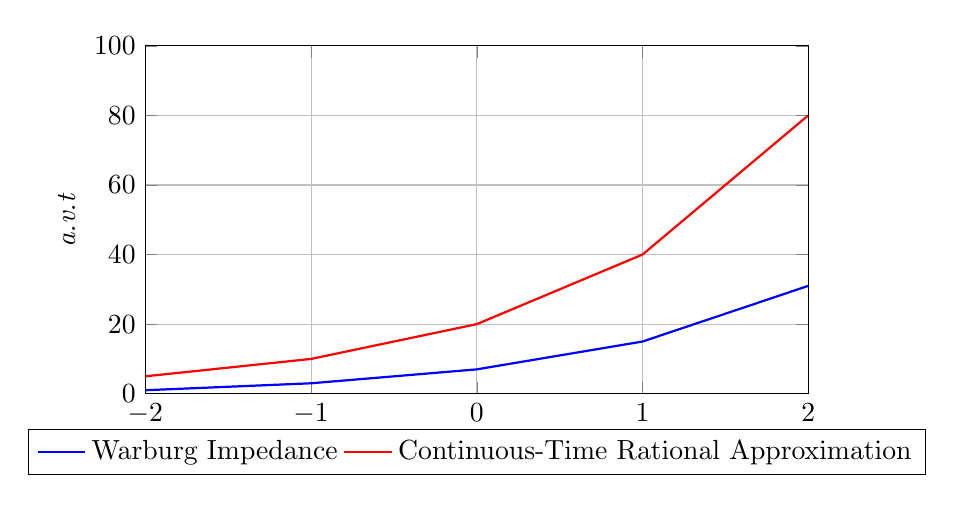
\begin{tikzpicture}
    \begin{axis}[
        width=10cm,
        height=6cm,
        xlabel={\textit{log }$z$},
        ylabel={\textit{a.v.t}},
        ymin=0, ymax=100,
        xmin=-2, xmax=2,
        log ticks with fixed point,
        ytick distance=20,
        xtick distance=1,
        grid=major,
        legend style={at={(0.5,-0.1)}, anchor=north,legend columns=-1},
        ]
        
        % Warburg Impedance (Blue)
        \addplot[blue, thick] coordinates {
            (-2, 1)
            (-1, 3)
            (0, 7)
            (1, 15)
            (2, 31)
        };
        \addlegendentry{Warburg Impedance}
        
        % Continuous-Time Rational Approximation (Red)
        \addplot[red, thick] coordinates {
            (-2, 5)
            (-1, 10)
            (0, 20)
            (1, 40)
            (2, 80)
        };
        \addlegendentry{Continuous-Time Rational Approximation}
    \end{axis}
\end{tikzpicture}
\end{document}